
\chapter{Materials and Methods}

In this thesis, three core-flooding experiments were conducted individually and summarised in Fig.\ref{exps}. The experimental methods will be described separately in the following sections. All experiments were conducted in ambient temperature 20$^{\circ}$C - 25$^{\circ}$C.

\begin{figure}[htbp]
  \centering
  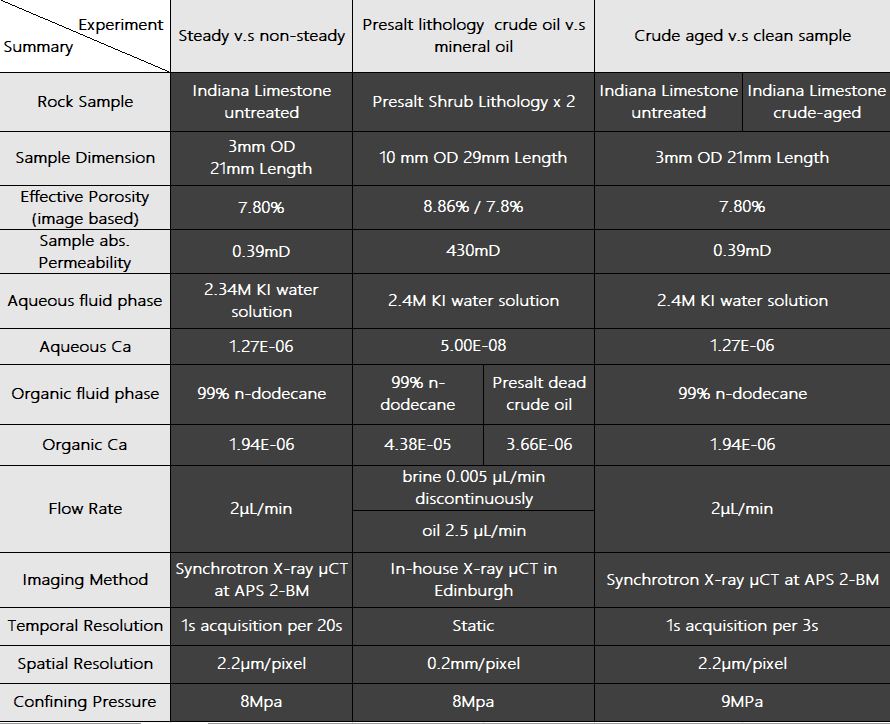
\includegraphics[width=1.2\textwidth]{\dir/figs/exps.png}
  \caption{Table: Summary of experimental conditions}
  \label{exps}
\end{figure}

\section{Experimental set I: Indiana limestone core-flooding experiments imaged with time-resolved synchrotron X-ray microtomography }
\label{2016}
\subsection{Year 2016 synchrotron experiments}
In these experiments, potassium iodide brine and mineral oil (99\% n-dodecane) were used as aqueous and organic fluid phase to perform core-flooding in an Indiana limestone (3mm OD by 21mm length) held in high pressure fluid flow cell 'Sleipnir'. Details of these experiments are listed in Fig.\ref{exps} first column steady v.s. non-steady experiments. These experiments were conducted by Drs Ian Butler and Marina Sousani prior to Yili Yang joined the project.

\subsubsection{Rock}
\paragraph{Indiana Limestone}
In the year 2016 time resolved synchrotron experiments, oolitic Indiana limestone samples were used as the porous rock media. SEM images of the samples (Fig.\ref{sempore}) illustrate two distinct surface topology, the rough, fine grained ooid surface, and the much smoother diagenetic drusy calcite cements surface (red circle in Fig.\ref{sempore}). The pore space magnitude has a wide distribution from under-micron to hundreds of microns. The micro pores that below the synchrotron X-ray microtomography resolution at APS (2.2\textmu m) are sub-resolution porosity that can not be identified by imaging, thus fluid flow inside these micro pores can not be detected and become one of the unavoidable limitations of this experiment. The total sample porosity was estimated of 20.65\% based on the ratio of measured sample density to pure calcite density. The porosity estimated by the ratio of pore to solid based on imaging was 6.5\%. The reasons for this discrepancy, is the sub-resolution porosity that can not be imaged that underestimate the porosity. The actual effective porosity should be higher than 6.5\%. The sample permeability was 0.39 mD, approximately estimated from a measurement of the pressure drop across the sample during loading with water.

The Indiana limestone sample is directly from outcrop and cleaned ultrasonically in de-ionised water in sample preparation.

\begin{figure}[htbp]
  \centering
  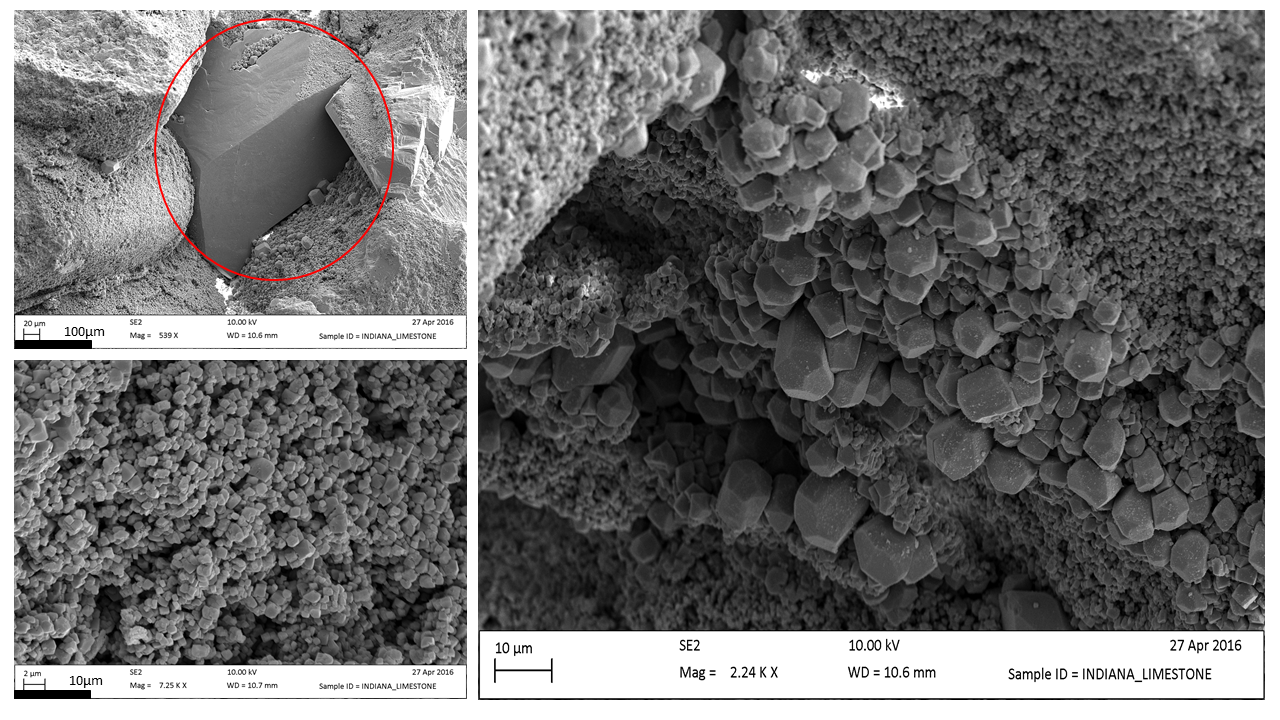
\includegraphics[width=1\textwidth]{\dir/figs/indianapore.png}
  \caption{SEM image of Indiana limestone: core surface with different scales from $100 \mu m - 10 \mu m$. Red circle shows different roughness of the surface. Pores of size close to $2 \mu m$ are close to the resolution of CT imaging used in this study therefore they are micro-pores that leads to underestimation of bulk porosity and uncaptured fluid flow.}
  \label{sempore}
\end{figure}
\paragraph{Core dimension}
The sample used in synchrotron experiments was sized 3mm OD by 21.2 mm length cylinder. The upper 13.7 mm (Fig.\ref{core} grey) was core end zone to exclude capillary effects from the volume of interest. The volume of interest is colored in green in Fig.\ref{core} (target zone), and for the volume above and below the target zone are the buffer zones where static scans were taken.

\begin{figure}[htbp]
  \centering
  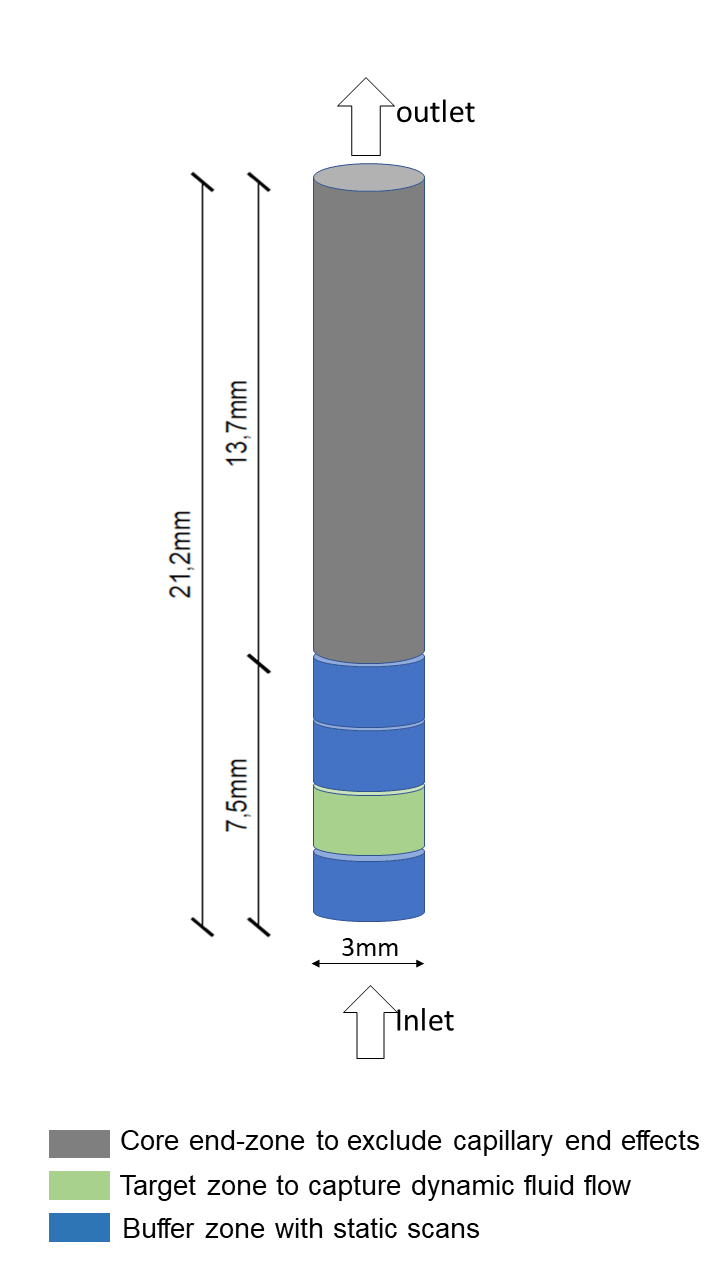
\includegraphics[width=.6\textwidth]{\dir/figs/core.png}
  \caption{Core dimension of Indiana limestone. The core used in the APS 2016 core flooding experiment. The dimension of the cylindrical core is 21.2 mm length $\times$ 3 mm diametre. The grey part of the core is space for eliminating capillary end effect. The bottom four blocks in blue and green are zones that being imaged for fluid flow processes. The blue zones are buffer zones which are imaged with static scans. The green zone is the target zone that imaged with fast scans to capture dynamic fluid flow processes.} 
  \label{core} 
\end{figure}

\subsubsection{Fluids}
\paragraph{Aqueous phase}
The aqueous phase was 2.4M Potassium Iodide (KI) water (deionized) solution. KI is a common doping agent for enhancing the X-ray imaging contrast with oil and rock \citep[e.g.]{iglauer2011residual,culligan2006pore,porter2010measurement}. The viscosity of KI solution at 25$^{\circ}$C is considered as close to water viscosity which is 0.89 MPaS reported by The International Association for the Properties of Water and Steam (IAPWS) 2008. The KI water solution is referred to as 'brine'.

\paragraph{Organic phase}
The organic phase for the synchrotron experiments is n-dodecane (99\%). Its solubility in water at 25$^{\circ}$C is reported to be 8.9 \times 10$^{-10}$ in mole fraction \citep{shaw2006iupac} and can be considered as immiscible with water. The viscosity of n-dodecane is reported in literature to be 1.36 MPaS at one atmosphere pressure and 25$^{\circ}$C \citep{liu2011measurement}. The density of dodecane $\rho=750$ kg/m$^3$ at ambient temperature. The interfacial tension of n-dodecane with water was reported to be 52.8 mN/m at 20$^{\circ}$C \citep{zeppieri2001interfacial}.

\subsubsection{Core-flooding cell}
\paragraph{'Sleipnir' cell}
The core-flooding cell used at synchrotron beamline APS 2-BM was 'Sleipnir' fluid flow cell described by \cite{fusseis2014low} (Fig.\ref{sleipnir2}). The cell was further modified for these experiments to include a carbon fibre composite pressure vessel to enhance X-ray transparency. In addition, the cell was partly re-engineered for zero-dead volume and fluid injections. The Sleipnir cell is capable of sample dimension up to 3mm diameter.

\begin{figure}[htbp]
  \centering
  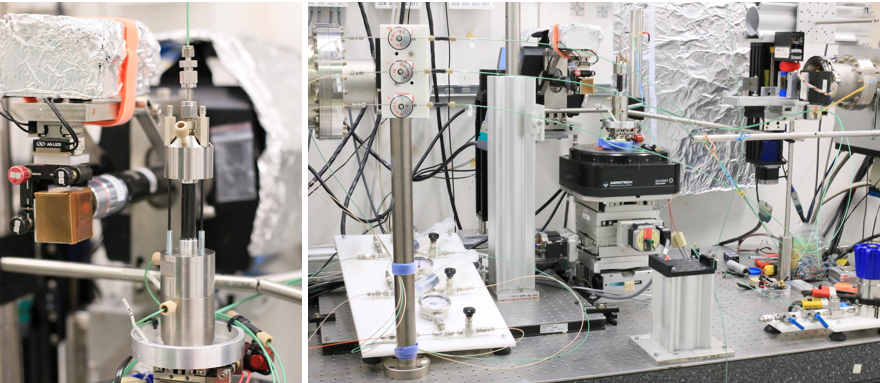
\includegraphics[width=.9\textwidth]{\dir/figs/sleipnir2.png}
  \caption{(Left) Sleipnir cell, with carbon fibre pressure vessel and tie-rods in place on the rotary table in the upstream hutch at 2BM, APS. (Right) Experimental set-up for two phase fluid flow, showing fluid manifolds, high pressure tubing (green). High pressure syringe pumps were located below the optical bench to shield them from scattered radiation. }
  \label{sleipnir2}
\end{figure}

\subsubsection{Core-flooding apparatus}
The experimental apparatus used in synchrotron facility consisted of fluid cell, syringe pumps, isolation valves, and a back pressure regulator (BPR). These components were connected by high pressure tubing and fluid manifolds (Fig.\ref{apparatus}). Three Cetoni neMESYS\texttrademark Syringe pumps were used to inject core-flooding oil, brine and confining fluid (water). The Syringe pumps were precisely controlled by software (Fig.\ref{apparatus} CETONI pumps). Three isolation valves controlled the flow of brine, oil and confining fluid which were leading into the fluid flow cell inlet (Fig.\ref{apparatus} flow cell). And a BPR controls the outlet pressure of the whole system and its outlet led to a waste-fluid bottle. 

\begin{figure}[htbp]
  \centering
  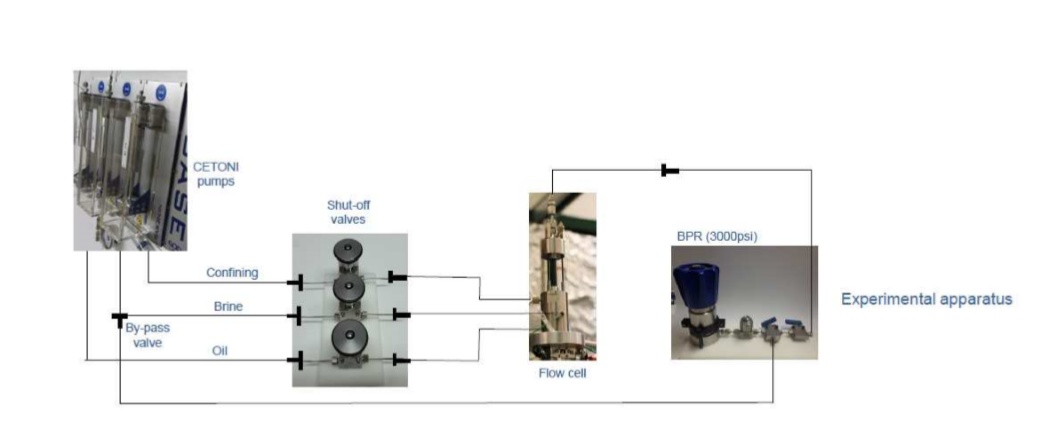
\includegraphics[width=1\textwidth]{\dir/figs/apparatus.png}
  \caption{ Experimental apparatus used at the APS facilities operating multiphase fluid flow experiments under elevated pressure. It consists of three syringe fluid flow pumps, three shut-off valves, a high pressure X-ray transparent fluid cell and a 6000psi back pressure regulator. Figure made by Dr.Ian Butler.}
  \label{apparatus}
\end{figure}

The inlet tube for steady state injections was designed as 'tube-in-tube' (Fig.\ref{design} cartoon) . This design consisted of a inner tube for oil flow and outer tube for brine flow. The design allows both fluids enter the core in a mixed fashion and reduced the impact of the location of accessed pores of fluid phases.

\begin{figure}[htbp]
  \centering
  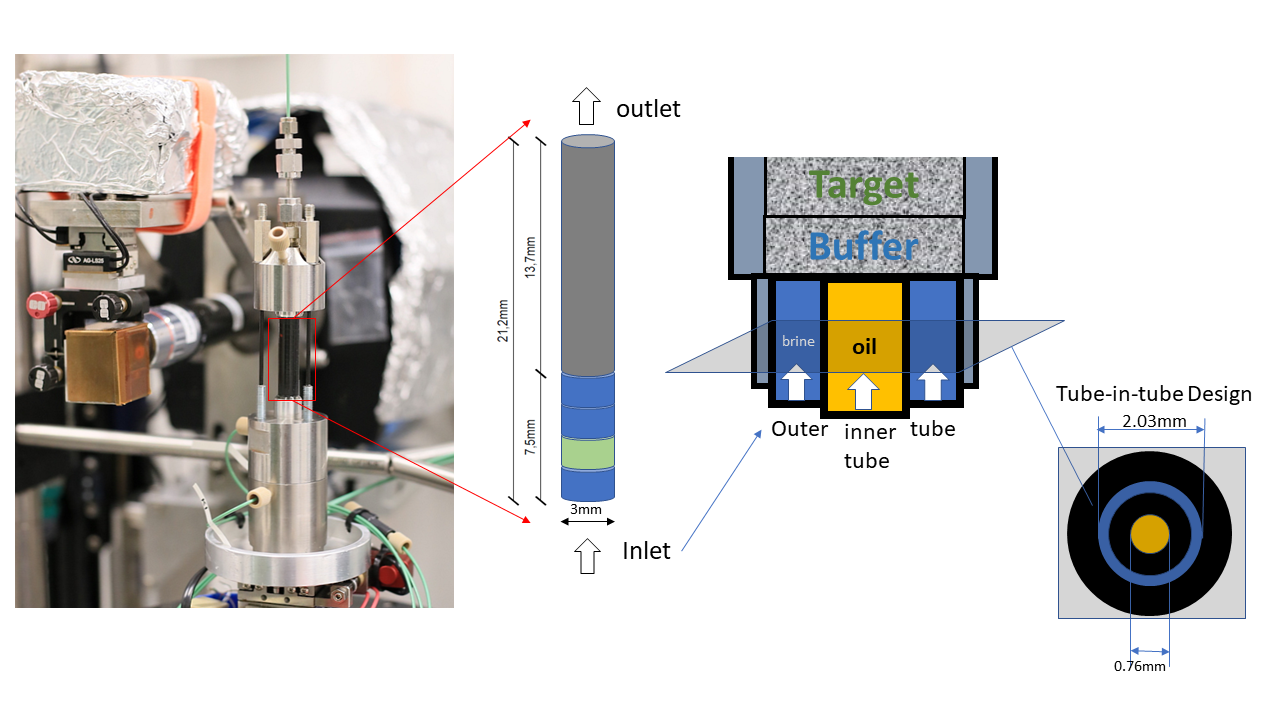
\includegraphics[width=1\textwidth]{\dir/figs/design.png}
  \caption{From left: Sleipnir cell, with carbon fibre pressure vessel and tie-rods in place on the rotary table in the upstream hutch at 2BM, APS. Red box zoomed in shows the carbon fibre vessel that holds the sample core. The inlet was designed tube-in-tube for oil and brine steady state injection. The cross-section of tube in tube design shows its dimension.}
  \label{design}
\end{figure}

\subsubsection{Experimental protocol}
\subsubsubsection{Core-flooding fluid injection sequence}
The Fluid injection sequence during core-flooding is summarised in table Fig.\ref{exptable}. The core before main core-flooding injections was saturated by water, then replaced by brine, then replaced by oil to an irreducible saturation. The experiment had three main stages:

\textbf{1) Brine injection (BI)} Brine injection into oil saturated core (Exp011-Exp015).

\textbf{2) Oil re-injection (OR)} Oil re-injection into brine saturated core (Exp017-Exp019).

\textbf{3) Steady state injection (SS)} Both fluids were injected simultaneously (Exp024-Exp027).

\begin{figure}[htbp]
  \centering
  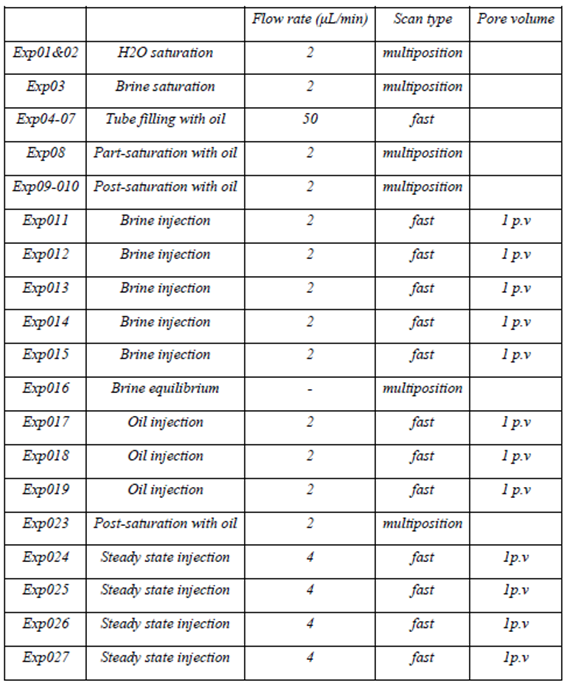
\includegraphics[width=1\textwidth]{\dir/figs/exp_table.png}
  \caption{Table: Sequence of fluid injections for the elevated pressure experiment}
  \label{exptable}
\end{figure}

\subsubsection{Imaging methods}
The experiments were imaged by synchrotron X-ray radiation at beamline 2-BM Advanced Photon Source (APS), Argonne National Laboratory, US.  This beam line is fully dedicated to fast imaging (second-scale) for slow dynamic phenomena studies. The synchrotron X-ray beam is sourced from the bending magnets that installed on the electron storage ring. The beam energy range is 11-35 keV and the beam size is 25mm x 4mm. Raw projection data was acquired by 2-BM internal code, and reconstructed by python based CT image processing library TomoPy \citep{gursoy2014tomopy}. TomoPy reconstruction is described in detail in the following Data Processing Methods section and TomoPy code written by Yili Yang is attached in the appendices.

The X-ray beam used for imaging is pink beam. Pink beam has narrower energy window comparing with white beam, combined with high photon flux can provide better contrast attenuation than white beam therefore yield higher quality CT images.

Three main injection stages were imaged by fast scans. During fast scan, 600 projections of 180$^{\circ}$ rotation were acquired for each tomogram. The exposure time for each projection was 1.7ms leading to 1s total acquisition time per scan. The gap between fast scans was 20 seconds. The spatial resolution is 2.2 micron per pixel. A total of 140+ CT volumes recording the fluid displacement processes were acquired at the end of experiments.

Multi-position scans were taken before and after each stage to check fluid position and acquire high resolution images. During Multi-position scan, 1500 projections of 180$^{\circ}$ rotation were acquired for each tomogram. The sample was moved vertically to make the x-ray beam scan multiple positions along the long axis of the sample.

\subsubsection{Data processing methods}
\paragraph{Overview}
The overall data processing for X-ray CT data includes reconstruction, segmentation, and post-segmentation analysis. The raw data acquired from X-ray CT are projection images. Reconstruction processes the projections into reconstructed data which are slices of horizontal sections of the object. Segmentation labels reconstructed images by meaningful categories such as pore and solid. The post-segmentation processes analyse the in-depth scientific features of the data. For example, calculates the connectivity of a fluid phase, or count the number and size of oil ganglions, or calculates the pore size distribution of a porous medium.

\subsubsubsection{CT reconstruction} 
The raw data acquired from an X-ray CT scan are the digital signals of attenuated X-ray photons converted into digital images called projections. The projections can be reconstructed to horizontal image section of the object by various of algorithms, e.g. filtered back-projection\citep{kak2002principles} , gridrec algorithm \citep{marone2012regridding,dowd1999developments} etc. By stacking the 2D reconstructed slices, 3D structure of the object can be digitalised.

\paragraph{Octopus}
Octopus\texttrademark is a commercial software for CT image reconstruction \citep{vlassenbroeck2006octopus}. It has a graphical user interface (GUI).  It uses filtered back-projection algorithm to perform reconstruction, and it includes image correction tool kits such as beam hardening correction, normalisation and denoise functions etc. It is user-friendly and faster for small batch of data. The reconstruction time for a CT volume sized $1600 \times 1600 \times 1000$ by Octopus usually takes around 40 minutes on a 16-core workstation. The latest Octopus version enables CUDA GPU acceleration so reconstruction time is massively reduced to few minutes. Octopus was used for the first 20 scans of the 2016 synchrotron experiments.

\paragraph{Tomopy}
TomoPy is an open-sourced software for CT image reconstruction \citep{gursoy2014tomopy}. It is python code based and does not have a GUI. The reconstruction functions include 13 major algorithms for instance filtered back-projection, Fourier grid-reconstruction, algebraic reconstruction and maximum-likelihood expectation maximization algorithm etc. It also includes other image correction functions such as auto centre finding, stripe removal functions, denoise filters and morphology functions. Because it is python based, it has several merits. First it is compatible with HDF files which is the standard data format for synchrotron data, while Octopus can not open. Second it allows user-defined pixel-wise operation, for the purpose of examining and fixing imaging errors. Thrid, it is compatible with other python software, like Open-CV \citep{opencv_library} and Scikit-image \citep{scikit-image}, to incorporate more useful functions and compose the best possible image processing work flow for unique data set. Fourth, it enables automatic batch processing that can loop different files in different folders and processing all-at once, which can save significant processing time. Fifth, it enables seamless subsequent processing of segmentation and scientific analysis using python.

Some parts of the synchrotron CT raw data have blank reconstruction slices, they were due to non-positive pixel values in the projection slices. During reconstruction, the values were proceeded as not-a-number (NaN) value when calculating minus-log function. The NaN value would raise problem resulted as blank slice. This problem was fixed by replacing all the non-positive value pixels in the projections by an extremely small positive number 1$^{-9}$.

The average reconstruction time for a CT volume sized $1600 \times 1600 \times 1000$ took less than a minute on a 32-core workstation. The majority of the synchrotron data was reconstructed by TomoPy. The TomoPy reconstruction code developed by Yili Yang can be found in the Appendices.

\subsubsubsection{preprocessing}
Raw CT reconstruction images usually have artefacts including noise, beam hardening and ring artefacts etc that make segmentation difficult. It is a common practice to pre-process the raw CT reconstruction images before segmentation to reduce the artefacts, thus to improve image quality and lead to better segmentation result. 

\paragraph{Cropping} The first step of pre-processing is cropping. Cropping is to re-size the raw image into the region of interest (ROI), and exclude the irrelevant background regions. Cropping can significantly reduce the processing time and computing resources needed, therefore it is the foremost step of all processing steps.

The following processing depends on the types of artefacts presented on the images. The common artefacts are random noise, ring artefacts, streak/stripe artefacts, beam hardening etc.

\paragraph{Noise} Random noise is the most common artefact, it is inevitable but relatively easy to be filtered. The reason of random noise can be various such as the fluctuations inherent in the detection of a finite number of x-ray quanta, additional signals created by electronic circuits during signal processing, or the round-off errors arise from binary computation \citep{hanson1981radiology}.

\paragraph{Non-local Means filter} 
In chapter two, a classical spatial filter, median filter is introduced. A more advanced filter, the non-local means (NLM) filter \citep{buades2011non} adopted the similar idea, but it replaces the given pixel with the weighted average value of the resembling pixels across the whole image, instead of the median of the peripheral pixels, because '\textit{the most similar pixels to a given pixel have no reason to be close at all}'. The resemblance is evaluated by comparing a square neighbourhood around each pixel, with intensity values and geometrical configuration both taken into consideration. The pixels on the boundary of objects are not averaged by their surrounding pixels, but restored by the pixel value with similar pattern - also on the boundary, therefore the noise is reduced meanwhile the boundaries are preserved. The mathematical expression of NLM is described as following equation:

$$NL[v](i)=\sum_{j\in i}w(i,j)v(j)$$

For pixel $i$ in noisy image $v$, the filtered pixel value $NL[v](i)$ is computed as the sum of weighted average of all resembling pixels $j$. The resemblance of $i$ and $j$ is measured as a decreasing function of the weighted Euclidean distance of their neighbouring values, meaning that the pixel with more similar neighbourhood has higher weight in the average. See \cite{buades2011non} paper for the complete mathematical description of the algorithm.

To compare the noise reduction performance on experimental CT data in this study, seven different filters are tested - the bilateral filter, total variation filter, Gaussian filter, Kuwahara filter, mean filter, median filter and non-local means filter. Non-local means filter has the best performance preserving edge features and noise reduction. And NLM filter has been widely implemented in ImageJ, Avizo\texttrademark and Scikit-image.

\begin{figure}[htbp]
  \centering
  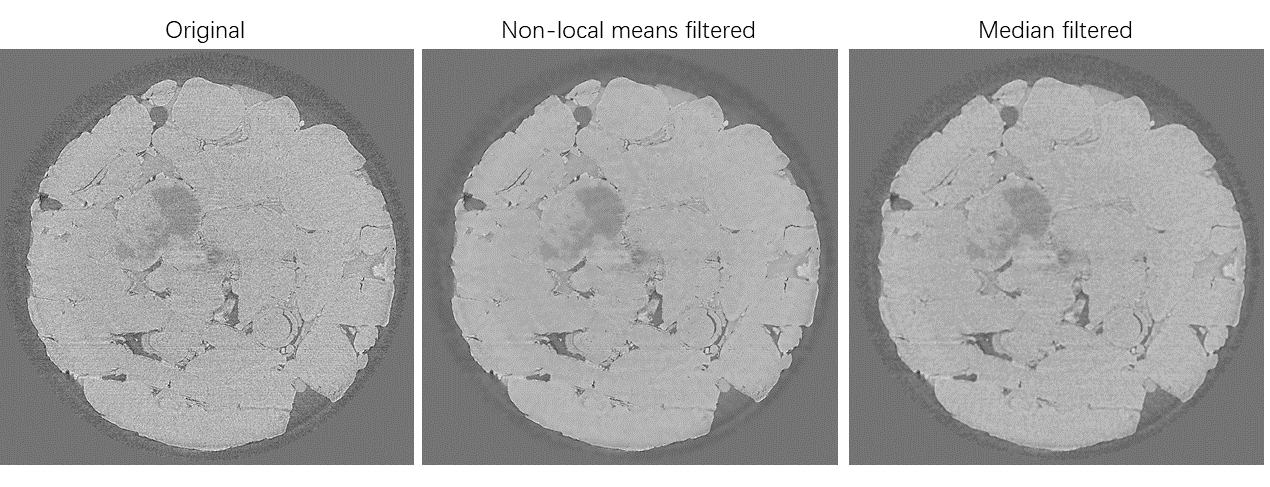
\includegraphics[width=1\textwidth]{\dir/figs/denoisecompare.png}
  \caption{Comparison of denoising by NLM and median filter}
  \label{denoisecompare}
\end{figure}

Fig\ref{denoisecompare} shows an example of comparison between NLM and median filter. The NLM filter has better performance on the example noisy image for less noise while preserving the sharpness of the phase boundaries. In Dr Tannaz Pak's PhD thesis \citeyear{Pak2014thesis}, she reported the comparison of median filter, anisotropic diffusion filter and NLM flter shows that NLM filter has the lowest standard deviation and the narrowest distribution peak in histogram. This confirmed the advantages of NLM filter for multiphase fluid flow experimental CT data in terms of noise removing while preserving phase boundaries.

Besides noise, a range of CT artefacts can be produced during the complex physical process and computing process of microtomography. Beam hardening , streak artefacts and ring artefacts can be alleviated by applying filtering algorithm during reconstruction. 

\paragraph{Intensity normalising} Synchrotron CT reconstructions can have problem that one CT volume have varied intensity along the vertical axis, i.e. some slices are overall brighter than others, and the degree of brightness varied across slices. This problem was fixed by normalising slices by their range of intensity.

$$ nmI(i)=\frac{i-I_{min}}{I_{max}-I_{min}}*a$$

In image $I$, the normalised pixel $nmI(i)$ of original pixel $i$ is calculated as the fraction of the intensity portion and the intensity range of image $I$. $I_{min}$ and $I_{max}$ are the minimum and maximum intensity in image $I$. The intensity portion of pixel $i$ is the difference of pixel value $i$ with the minimum intensity $I_{min}$. The intensity range is the difference of maximum and minimum intensity. $a$ is a coefficient, when $a=1$ the normalised output image format is floating point ranged from 0-1. When $a=255$ the normalised output image format is 8-bit unsigned.

In the 2016 synchrotron experiments, the contrast between the solid phase and aqueous phase is subtle, even with 2.34M KI contrast enhance doping added to the aqueous phase. In order to segment the image, a masking pre-process was applied. A binary segmentation of soild and pore space was extracted from the reference scan at time zero. The segmentation of solid was employed as a mask for the subsequent segmentation of multiphase fluid flow process. (img) 

\subsubsubsection{Segmentation} 
Accurate and efficient image segmentation is the crucial prerequisite of quantitative analysis on CT images. Image segmentation is to assign meaningful labels to digital images pixel-wisely, for example giving each pixel a label of oil, brine or solid to a multiphase fluid flow core-flooding X-ray image. Due to great amount of CT data produced in the experiments and the complexity of the image pattern, it is impossible to manually segment the images. Therefore it is crucial to find an accurate and efficient method to segment CT images.

Conventional segmentation algorithms such as Otsu thresholding \citep{otsu1979threshold} or watershed segmentation \citep{serra1983image} are widely used in the image processing of multiphase flow experiments \citep[e.g.]{andrew2015imaging,singh2016imaging}. In this study, a more advanced algorithm - Seeded Random walker (RW) segmentation \citep{grady2005multilabel} is employed to segment the experimental CT reconstruction images. Random walker is a region growing algorithm similar with watershed, but with better performance in terms of accuracy and efficiency, it also provides probability map for a quantitative evaluation of the segmentation reliability.

\begin{figure}[htbp]
  \centering
  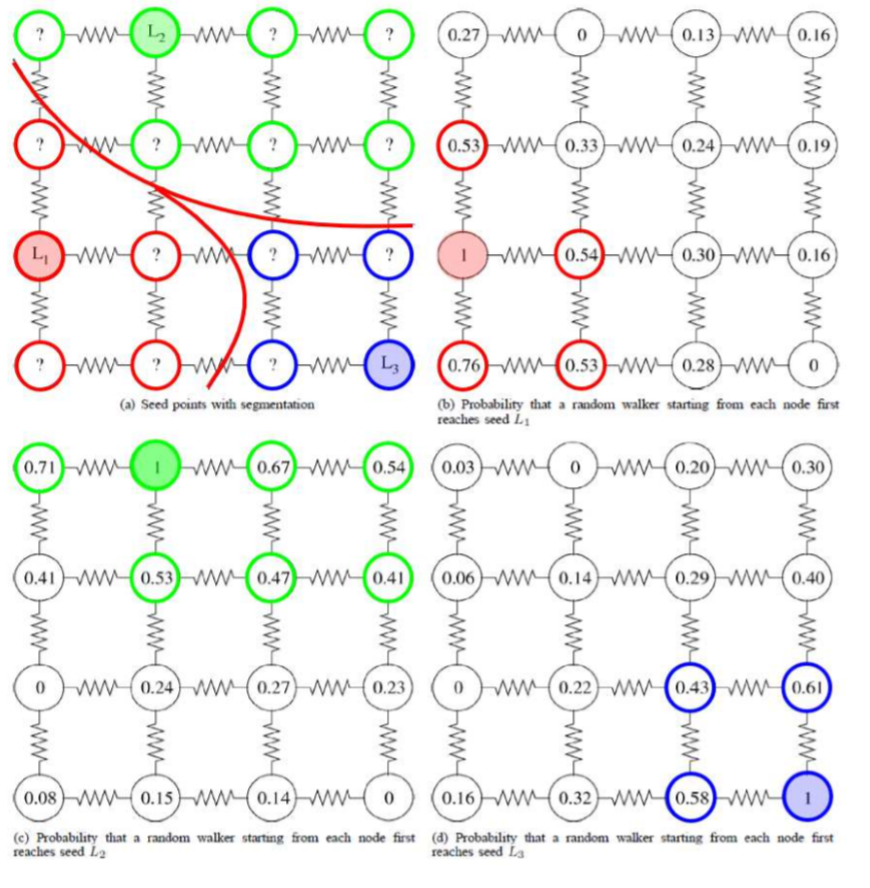
\includegraphics[width=1\textwidth]{\dir/figs/rw.png}
  \caption{An illustrative example of a random walker segmentation (a) modified by Dr Ian Butler from Grady (2006). In this example Grady (2006) uses fixed nodes connected by resistors, with the marker nodes, L1, L2 and L3, alternately (b, c, \& d) representing nodes fixed to a potential of 1 and all resistors were set to the same value. The electric potentials calculated represent the probability that a random walker starting at each node first reaches the seed point currently set to unity. The colour codes indicate which nodes with the highest values “belong” to which marker point, and the final segmentation is shown in (a) as the red line. Translating this example to the case of an image, each resistor would represent a function of the grey scale gradient in the image}
  \label{rw}
\end{figure}

\paragraph{Random Walker Segmentation}
The seeded random walker algorithm was motivated by placing small number of user-defined labels (seeds) that unequivocally belong to a particular phase (i.e. solid), and perform random walk from pixels then noting which seed they first arrive at. Random walk is one of the famous problem scenario in probability theory that a man walking on a street and making turn by probability, and well known for its equivalence with electrical circuits \citep{doyle1984random}. In this algorithm, random walk is performed at each unclassified pixel and noting the probability that they arrived at each seed, and is categorised to the seed with the highest probability. The mathematical problem was solved by combining probability theory and circuit theory on a graph. The image structure was represented by a function that map pixel intensity to edge weights that affect random walker's choice.  

Fig.\ref{rw} shows the analogue of random walker segmentation to electric circuits: the electrical nodes (pixels) are connected by resistors (weights) to the voltage source (seeds) L1, L2, L3 in (a). By solving the probability problem with the aid of circuit theory, the electric potentials (segmentation probability) is computed, and the segmentation is determined by the highest probability.

Random walker algorithm is highly robust that unlikely suffer from the three usual problems in CT image segmentation 1)corrupted image with noise and artefacts, 2)different objects with low contrast or absent boundaries and 3)ambiguity of labels when they are fewer than constant regions. 

\begin{figure}[htbp]
  \centering
  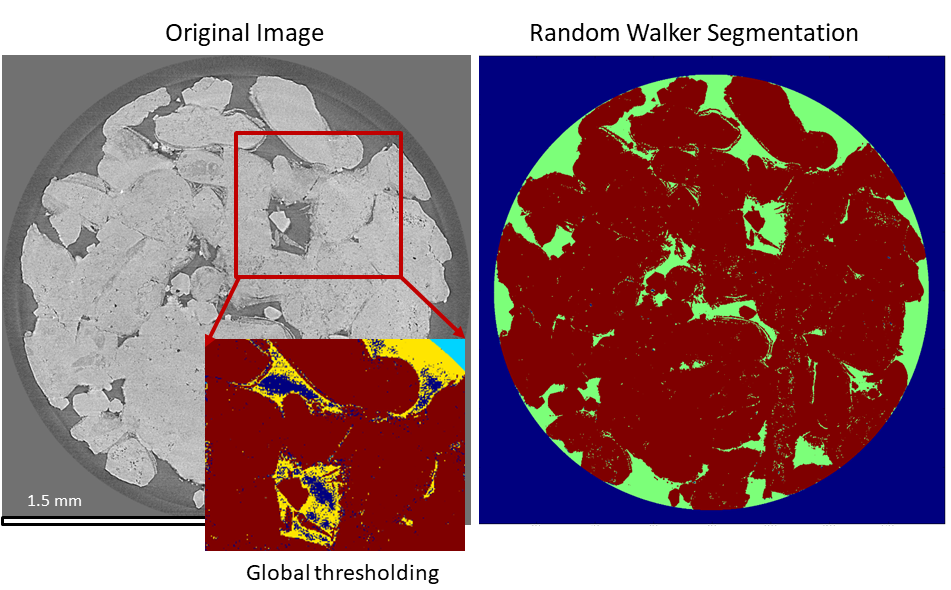
\includegraphics[width=1\textwidth]{\dir/figs/rwresult.png}
  \caption{Random walker segmentation example result}
  \label{rwresult}
\end{figure}

Fig.\ref{rwresult} shows the original reconstructed CT image and the random walker segmentation result that separating pore space and solid. Zoomed-in red box on the original image shows The global thresholding result, blue speckles are the pixels with intermediate intensity that can not be thresholded. The random walker segmentation shows a sharp and clean segmentation of the pore and solid, this high quality segmentation is used as mask for the segmentation of experimental data with two fluids present in the pore space.

Fig.\ref{segworkflow} shows the work flow of segmentation. The raw image is severely suffered from noise and the contrast between solid and brine is poor. By applying mask obtained from Fig.\ref{rw} on the raw image, the masked image shows the to-be-segmented pore space saturated with oil and brine. By applying non-local means filter, the noise is massively reduced and ready for RW segmentation. The seeds are determined by histogram, and the final segmentation is performed by seeded RW implementation in Scikit-image. The segmentation code developed by Yili Yang is attached in the Appendices chapter. The processing work flow took average one hour for each CT volume sized $1646 \times 1646 \times 1004$. A total of 140 plus volumes of synchrotron CT data was segmented using this method.

\begin{figure}[htbp]
  \centering
  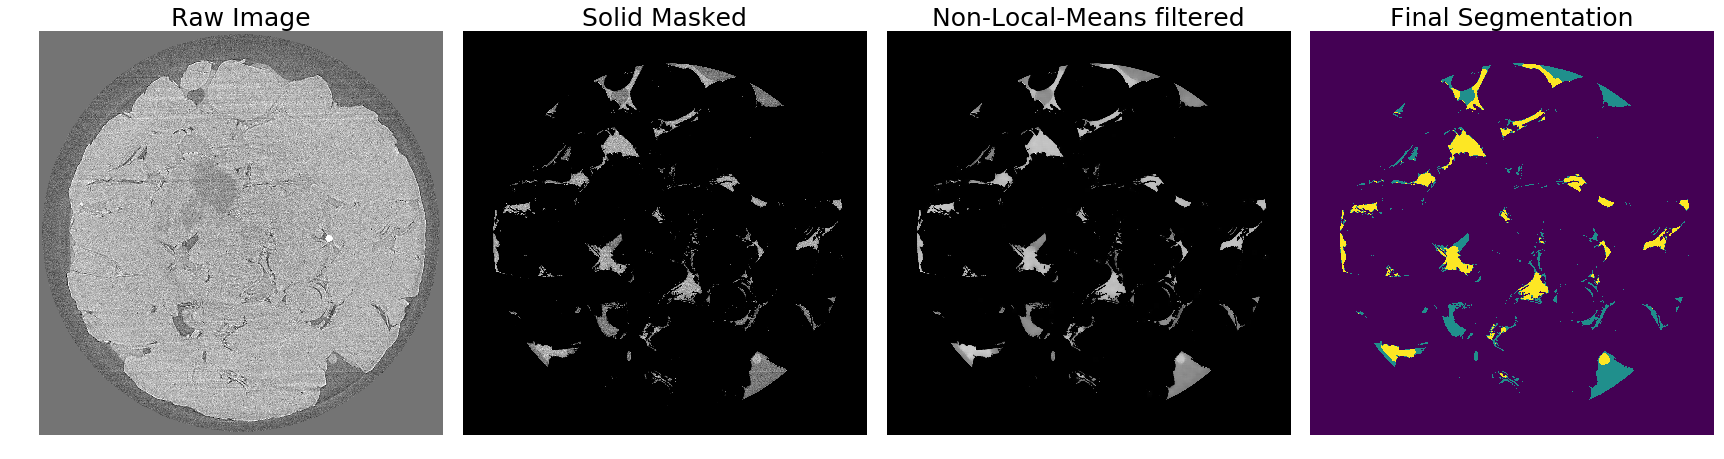
\includegraphics[width=1\textwidth]{\dir/figs/f.png}
  \caption{Segmentation work flow}
  \label{segworkflow}
\end{figure}

Fig.\ref{seg2} shows a comparison of the same slice before and after injection, and the segmentation result of injection fluids. Left image shows the reference water-saturated core prior to experimental injection, the image was acquired from static scan which has higher resolution than fast scans. A precise segmentation of solid and pore space is acquired from this image. Middle image shows the fast scan image of the same slice during brine injection. The fast scan achieved high temporal resolution at the cost of compromised image quality. The fast scan image has more noise and horizontal stripe artefact, more importantly, the contrast between brine and solid is so poor that can be barely visually identified. After the segmentation work flow, accurate segmentation of the two fluid occupied pore space and solid is shown on the right. 

\begin{figure}[htbp]
  \centering
  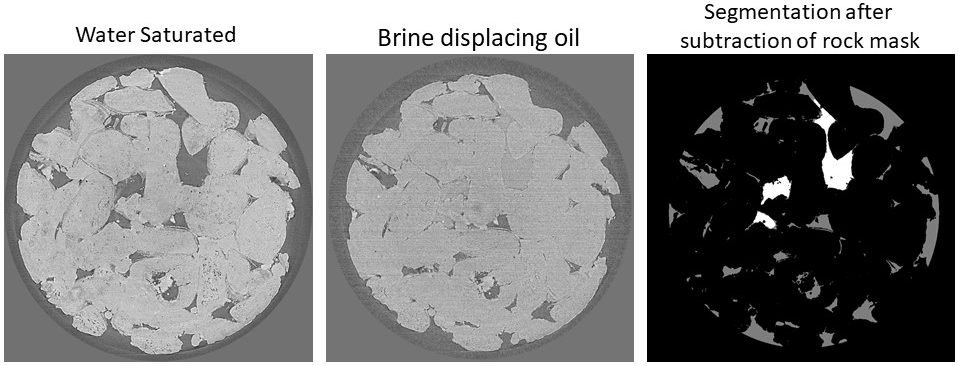
\includegraphics[width=1\textwidth]{\dir/figs/seg2.png}
  \caption{Segmentation result}
  \label{seg2}
\end{figure}

The RW segmentation probability map is shown in Fig.\ref{probmap}. It visualise the probability distribution of all pixels on a image belong to a particular phase. The original image is shown on the left, middle and right images are the segmentation probability distribution of solid and pore space (filled with H$_2$O) respectively.
The colour map is scaled from 0-1 from colour cold to warm. For the probability value of each pixel on the map, the more close to 0 means the lower likelihood that it belongs to the target phase and vice versa. The uncertainty lies in those pixels with likelihood around 0.5, meaning that it is hard for the algorithm to decide whether this pixel belongs to a particular phase or not. The maps in Fig.\ref{probmap} show a very robust segmentation with many determined pixels and only few uncertainty.

\begin{figure}[htbp]
  \centering
  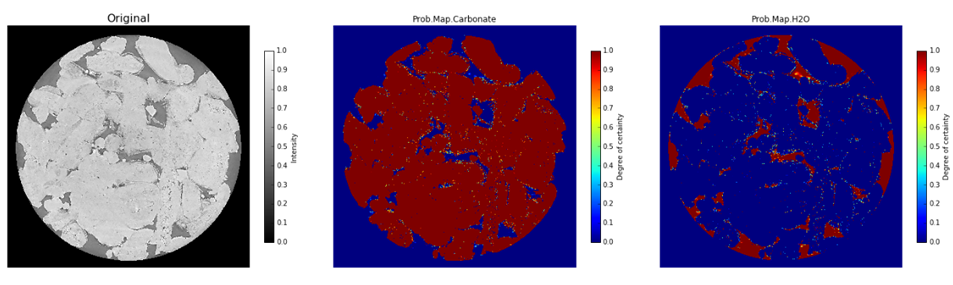
\includegraphics[width=1\textwidth]{\dir/figs/probmap.png}
  \caption{Probability map produced by random walker algorithm}
  \label{probmap}
\end{figure}

Accurate segmentation of CT images guarantees that experimental phenomena are honestly digitalised. Only then can we analyse the physical process presented in the experiments. 

\subsubsection{Post-segmentation image processing}
\subsubsubsection{Fluid connectivity estimation using Euler characteristics}

To study the connectivity evolution of fluid phases during displacement, Euler characteristics ( Euler--Poincar\'e characteristic) is employed as a measurement of topological connectivity of fluid phases. 

The topological definition for a three-dimensional object can be described using Minkowski functionals (details see \cite{blunt2017multiphase,mecke2005fluids}). There are four functionals: M$_0$ the volume of the object, M$_1$ the total area of the object surface, M$_2$ the average curvature on the surface and M$_3$ the total curvature of the surface. M$_3$, unlike the first three functionals, is dimensionless and related to the Euler characteristic $\chi$, which describes the relationship between the number of edges, faces and vertices of a polyhedron,

$$\chi = V-E+F-O$$,

where V is the number of vertices, E the number of edges, F the number of faces and O the number of discrete objects. To relate $\chi$ to the measure of connectivity, this relation is generalised \citep{serra1986introduction,vogel2001quantitative,vogel2002topological} to: 

$$\chi=\beta_0-\beta_1+\beta_2$$,

where $\beta_0$ is the zeroth Betti number referring to the disconnected discrete regions of the object, in the context of this study $\beta_0$ is the individual fluid ganglions and clusters. $\beta_1$ is the first Betti number referring to redundant handles or loops that can be eliminated without breaking the connectivity, quantified by $\beta_0$ staying constant. In the experimental context $\beta_1$ is the pores multiply interconnected by throats. $\beta_2$ is the 2nd second Betti number referring to isolated regions surrounded inside the object. In the experimental context it is the non-wetting fluid completely trapped in a pore surrounded by the wetting fluid.

The Euler characterestics (simplified as Euler number) for the fluid phases were computed using Avizo9\texttrademark. The Euler number is normalised with fluid volume to characterise the unit volume connectivity of the phase.

\subsubsubsection{Pore size distribution}
Pore size distribution (PSD) is an important characteristic of a porous medium. It describes the pore population in relationship with pore width in a porous medium. The PSD of a porous medium can be experimentally determined using many methods including molecular adsorption method (molecular resolution porosimetry), small angle X-ray scattering, mercury porosimetry, nuclear magnetic resonance, thermoporosimetry, liquid extrusion porosimeter, size-exclusion chromatography, water vapor desorption isotherms etc \citep{kaneko1994determination, yang2009image}. From an image-based perspective, PSD can be determined by max ball method or porosimetry simulation etc \citep[e.g.]{delerue1999new,yang2009image,gostickporespy}. 

In this study we used a local thickness approach implemented by \cite{gostickporespy} in python. The algorithm calculates the largest engulfed sphere for each voxel in an image and returns a copy of that image with the pore size value in each voxel. With this image mapped with pore size value, we can plot the PSD curve for different porous media. 

\begin{figure}[htbp]
  \centering
  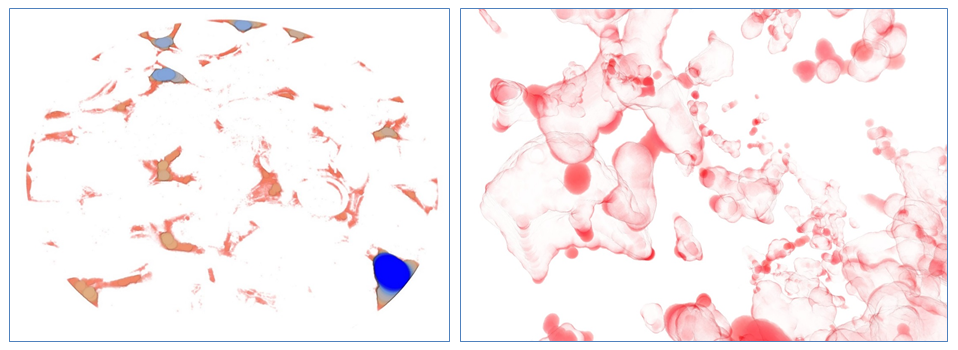
\includegraphics[width=1\textwidth]{\dir/figs/localthickness.png}
  \caption{Visualisation of maximum engulfed sphere in 2D and 3D}
  \label{localthickness}
\end{figure}

Fig.\ref{localthickness} left shows an image slice produced by local thickness function, the pores are filled with spheres that indicate the maximum radius of that pore, and PSD of the 3D porous medium can be plotted from all the slices. Image on the right shows the 3D rendering of pores with certain size range rendered with red, pores out of this range are not rendered and transparent.

\subsubsubsection{Pore throat-body partitioning}
The size of pore is a fundamental control on the fluid flow process. According to the Young-Laplace equation, it is more energy favourable that wetting phase occupying the narrowest regions first, which means the throats are easy to flow and the pore body impedes the flow. And vice versa for non-wetting phase. In order to know the wettability of the porous medium, as contact angle measurements for every throat that fluids were passing by is not easy, it is more practically feasible to compare the size of pores that fluids were passing by to estimate the wettability.

In this study I established a method to compare the throat size that passed by a fluid with those unpassed throats quantitatively. If a fluid phase passed more larger throats than smaller throats, this fluid phase is generally non-wetting to the porous medium, and vice versa.

\begin{figure}[htbp]
  \centering
  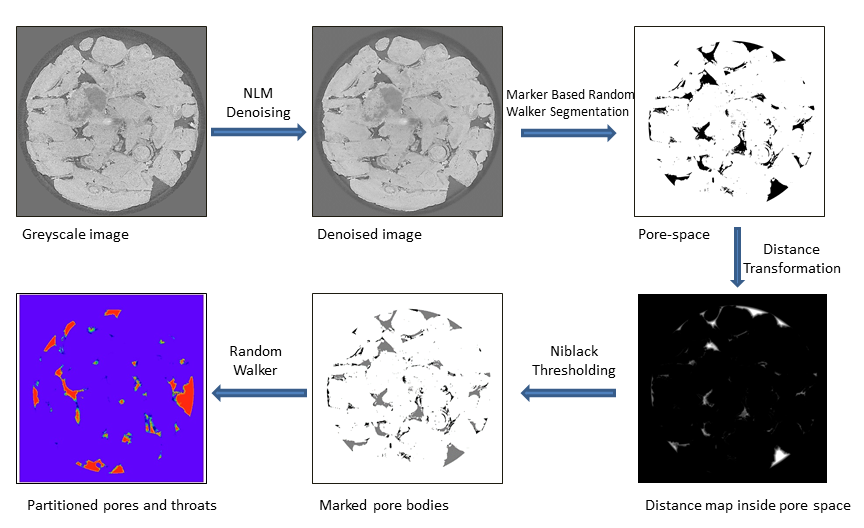
\includegraphics[width=1\textwidth]{\dir/figs/partitionwf.png}
  \caption{Pore body-throat partitioning work flow}
  \label{partitionwf}
\end{figure}

The method work flow is shown in Fig.\ref{partitionwf}. First the raw CT image (1) is denoised (2), and segmented into a binarilised pore space (3). Then Euclidean distance map (4) of the pore space is computed, which is the Euclidean distance of a pixel to its nearest boundary, i.e. the distance of a point inside the pore to the closest rock surface. This distance map is then thresholded using Niblack thresholding \citep{niblack1985introduction}, to find the local maxima of the distance map. The local maxima represent the widest areas locally, which are pore bodies. The unthresholded area in (5) are the throats, the narrowest areas locally. By applying random walker probability map to (5), throats are labelled with the likelyhood of belonging of its nearest pore body (6). 

\begin{figure}[htbp]
  \centering
  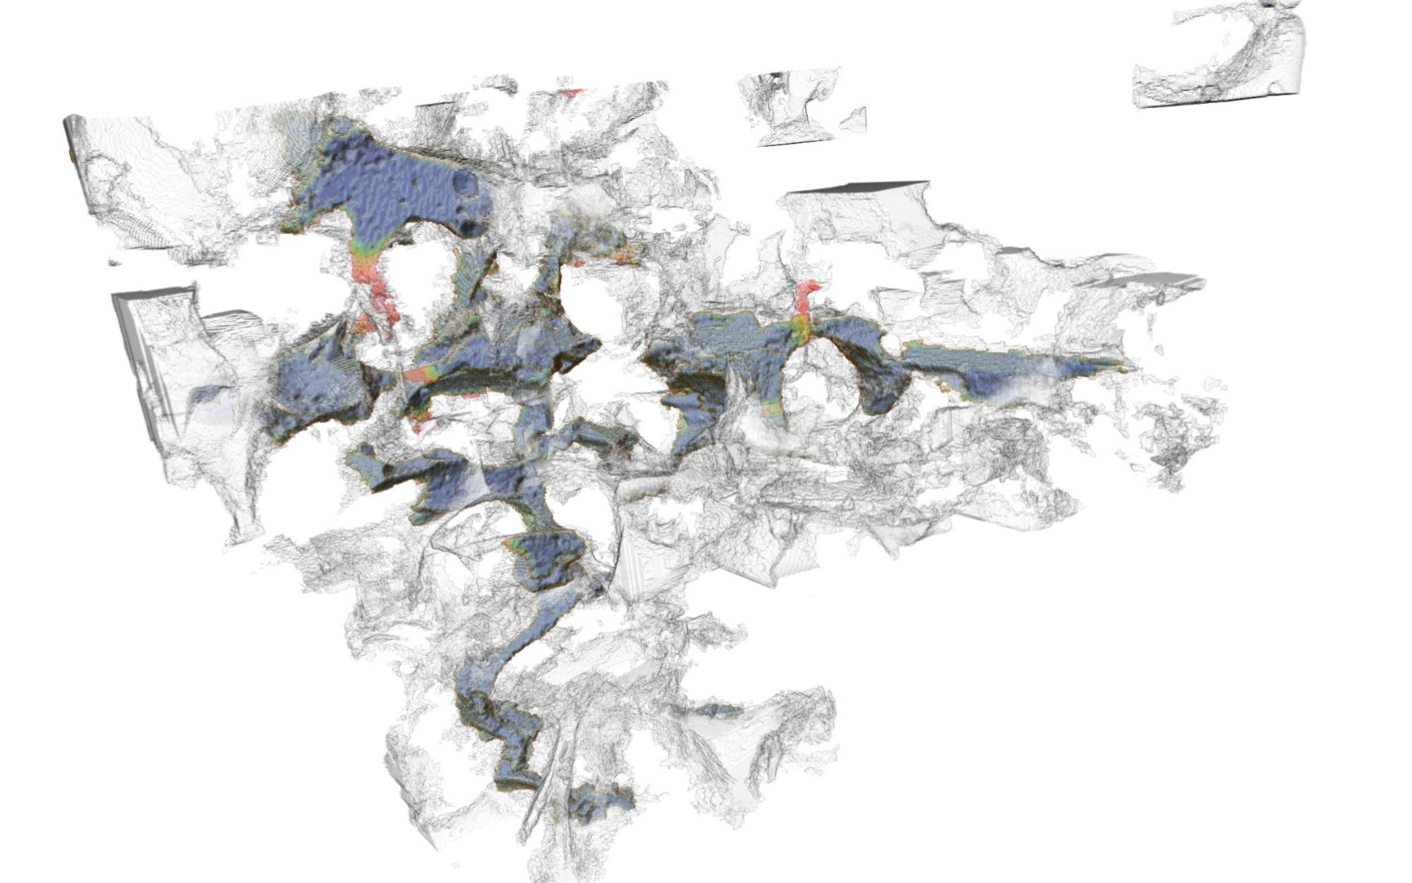
\includegraphics[width=1\textwidth]{\dir/figs/throats.png}
  \caption{3D rendering of brine passing throats labelled in colour}
  \label{throats}
\end{figure}

Fig.\ref{throats} visualised the brine inside the oil saturated pore and the pore bodies and throats are rendered from cold to warm colour. This allows a intuitive observation of sizes of throats and pores that fluids were passing.

The most important application of this method is to quantify the size of throats that fluids were passed or unpassed (Fig.\ref{throatsize}). By comparing two adjacent scans in a time series, the throats that connected with the fluid occupation can be examined if they were passed or not. In this figure of throat size distribution, brine passed throats (green) has a positive offset with unpassed throats (red), meaning that brine favours larger pores in general, but still passed some smaller throats, indicating that for the examined region, the porous medium is largely non-wetting to aqueous phase.

\begin{figure}[htbp]
  \centering
  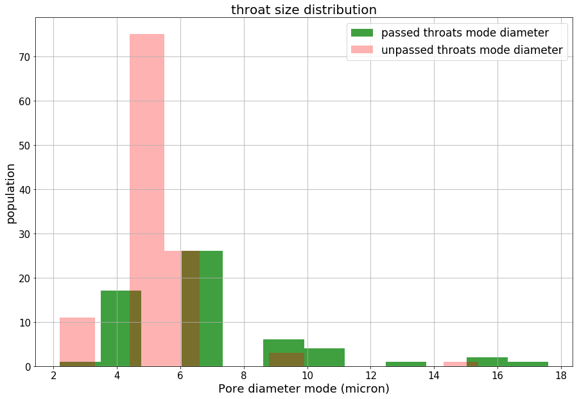
\includegraphics[width=1\textwidth]{\dir/figs/throatsize.png}
  \caption{Passed and unpassed throat size distribution}
  \label{throatsize}
\end{figure}

\subsubsubsection{Modelling of a Roof-snap off event}


%%%%%%%%%%%%%%%%%%%%%%%%%%%%%%%%%%%%%%%%%%%%%%%%%%%%%%%%%%%
\subsection{Year 2017 synchrotron experiments}

In these experiments, brine and mineral oil (99\% n-dodecane) were used as aqueous and organic fluid phase to perform core-flooding in a crude-aged Indiana limestone and an unaltered Indiana limestone (3mm OD by 21mm length). The aim of these experiments is to compare the fluid flow process in crude-aged and unaltered carbonates. Details of these experiments are listed in Fig.\ref{exps} third column.

\subsubsection{Rock}
The cores used in this experimental series are sub-sampled from the same Indiana limestone main sample used in year 2016 synchrotron experiments. Detailed description of this sample see section \ref{2016}.

One Indiana limestone sub-sample was aged with crude oil from Presalt Lula Field to alter its wetting properties. Dead crude oil was introduced into the sample by micro-centrifugation, the oil-covered sample was then kept for 54 days at 75$^{\circ}$C. The pore surfaces can adsorb polar components in the crude oil and thus change its wetting properties \citep{buckley1998mechanisms}. This sample is referred to as crude-aged sample. Another Indiana limestone sub-sample remained untreated as control group, and referred to as unaltered sample.
\subsubsection{Fluids}
\paragraph{Aqueous phase}
The aqueous phase used was the same KI solution as year 2016 synchrotron experiments.
\paragraph{Organic phase}
The organic phase used was the same n-dodecane (99\%) as year 2016 synchrotron experiments.
\subsubsection{Core-flooding cell}
The core-flooding cell used was the same cell 'Sleipnir' used in year 2016 synchrotron experiments, except that the tube-in-tube and zero dead-volume injection design was abandoned.

\subsubsection{Core-flooding apparatus}
The core-flooding apparatus used was the same as year 2016 synchrotron experiments.
\subsubsection{Experimental protocol}
\subsubsubsection{Fluid injection sequence of unaltered Indiana limestone sample}
1) H$_2$O flood and brine saturated pre-injection

2) Dodecane injection 

3) Brine re-injection
\subsubsubsection{Fluid injection sequence of crude aged Indiana limestone sample}   
1) Dodecane saturated pre-injection

2) Brine injection

In the crude-aged sample experiments, data acquisition was halted after step 2)brine injection due to camera malfunction, we were unable to continue with further injections.


\subsubsection{Imaging methods}
The technical aim of the experimental suite is to achieve higher temporal resolution synchrotron micro tomography than 2016. We imaged the experiments in beam line 2-BM Advanced Photon Source (APS), Argonne National Laboratory, US. 

Imaging was performed using pink beam radiation. High quality reference scan of 1500 projections was acquired pre-injetion. The dynamic process of fluid flow was imaged by fast scan of 600 projections through a 180$^{\circ}$ rotation in one second. The interval between each scan was 3 seconds, which is seven times faster comparing with the 20 seconds interval achieved in 2016.  The rotation of the rotary stage, where the sample was mounted, is synchronised with the camera. This allows data acquisition during the rotation of the sample in clockwise and anticlockwise, rotational acceleration and de-acceleration. Zero-dead volume tube-in-tube fluid delivery method using in 2016 was abandoned to minimise the tubing attached which can block the beam. In total over 500 \textmu CT volumes were acquired. 

\subsubsection{Data processing methods}
\subsubsubsection{CT Reconstruction}
Raw CT projections were reconstructed by applying Tomopy CT reconstruction script developed by Yili Yang.

%#################################################################################
\section{Experimental set II: Presalt lithology core-flooding experiments imaged with in-house X-ray microtomography}

In these experiments, brine, mineral oil (99\% n-dodecane) and crude dead oil from Presalt Lula field were used to perform core flooding in a Presalt shrub lithology sample core, held in cell 'Slidr'. The experimental details are summarised in Fig.\ref{exps} second column.

\subsubsection{Rock}
Presalt shrub lithology sample F4402H (Soxhlet cleaned) from Lula Field was cored into two cylinder sub-sample cores of 10mm OD and 29mm length (Presalt Lula LL-1D-RJS, Depth: 5073.35 m, Absolute Permeability: 430 mD, Effective Porosity: 7.8\%; Density: 2.7 g/cm$^3$). Two sub-samples were cored from this main sample to perform dead crude oil injection and mineral oil injection.

\subsubsection{Fluids}
\paragraph{Aqueous phase}
The same KI solution as year 2016/2017 synchrotron experiments was used in this experimental set.

\paragraph{Organic phase}
Dead crude oil from Presalt Lula Field was used in the Presalt shrub lithology sample F4402H experiments using in-house X-ray \textmu CT. Dead oil refers to oil that has lost its volatile components. Interfacial tension of this dead crude oil with water was estimated to be 20 mN/m by Dr.Surmas Rodrigo from Petrobras. Viscosity (NS/m$^2$) at 20$^{\circ}$C is estimated to be 0.043 by curve fitting Petrobras lab measurements at higher temperatures (Fig.\ref{viscosity}).

\subsubsection{Core-flooding cell}
\paragraph{Cell 'Slidr'}
The large sample core-flooding cell (Fig.\ref{largecell3}) is known as ICCR microtomography flow cell 'Slidr', comparing with Sleipnir, can accept sample dimension up to 10mm OD and 40mm length and elevated pressure. We used this cell for larger samples imaged by Edinburgh in-house X-ray \textmu CT. This cell is made of carbon fibre and steel. It has been tested to 20MPa (3000 psi) confinning pressure and designed parameters indicate safe operation up to 35Mpa. Its dimension enables larger sample size thus can study more heterogeneous carbonate rocks. The cohesion material used in this core constrains the temperature limit to 40$^{\circ}$C. The cell was designed by Dr. Ian Butler and manufactured in the workshop in School of Geoscience, University of Edinburgh.

\begin{figure}[htbp]
  \centering
  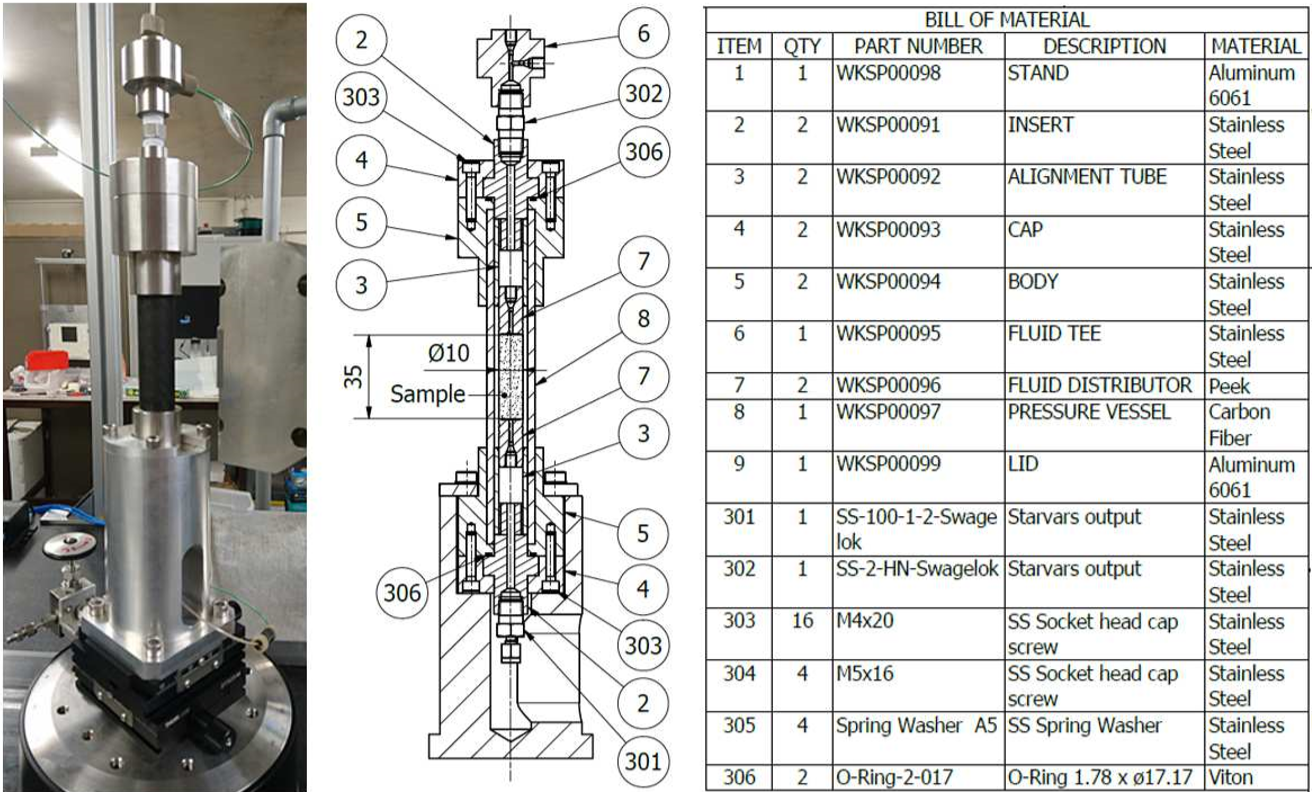
\includegraphics[width=.9\textwidth]{\dir/figs/largecell3.png}
  \caption{(Left) The flow cell ‘Slidr’ installed on the rotary table of the University of Edinburgh’s micro-tomography instrument. (Middle) Cross section through the cell and cell stand. The cell uses a tube in tube design to enable confining and pore fluid access via the end caps. (Right) The bill of materials for the cell. Stainless steel (316) offers excellent machine ability and corrosion resistance, however CP2 titanium is an alternative that would offer sufficient strength and corrosion resistance and reduce the overall mass of the cell.}
  \label{largecell3}
\end{figure}

\subsubsection{Core-flooding apparatus}
The experimental set-up was as illustrated in Fig.\ref{inhousect} and conditions were confining pressure = 80 bar (8 MPa), and fluid outlet pressure was set using a back pressure regulator to 53 bar (5.3 MPa). All processes were conducted at ambient temperature.

\begin{figure}[htbp]
  \centering
  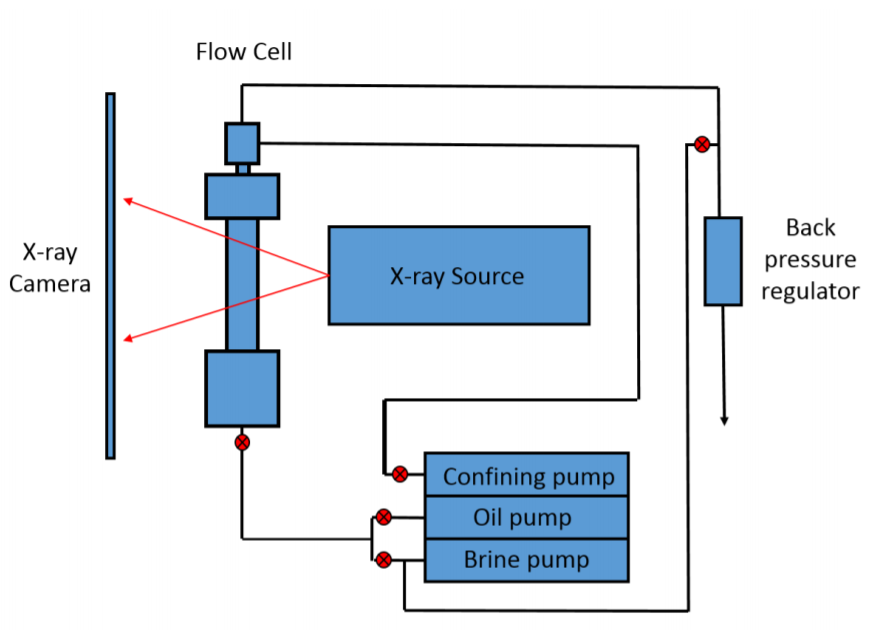
\includegraphics[width=.9\textwidth]{\dir/figs/inhousect}
  \caption{Experimental set-up for core-flooding experiments. Image adapted from ICCR final report 2019.}
  \label{inhousect}
\end{figure}

\subsubsection{Experimental protocol}
\subsubsubsection{Fluid injection sequence using dead crude oil}
The overall experimental sequence is summarised as follows: 

1) Water saturated scan pre-injection

2) Displace water with brine 

3) Brine saturated scan 

4) Dead crude oil injection for 4 pore volumes (2.5 \textmu L/min) 

5) Dead crude oil saturated scan 

6) Brine re-injection (0.005 \textmu L/min discontinuously)

7) Multiple scans, partially brine to saturated conditions

The first set of experiments the oil used is dead crude oil from Presalt Lula field. During Brine re-injection (step 6), displacement of previously injected dead crude oil by brine resulted in a significant inlet pressure rise, even when flow rates were reduced to the minimum rate of the pump (0.005\textmu L/min). We had to halt brine injection when inlet pore fluid pressure approached 70 bar, and waited for inlet pressure slowly reduce. The reason of this pressure rise is currently unknown, it may related to the temperature we were performing. According to Dr Surmas Rodrigo from Petrobras, this dead crude oil can flow smoothly in the core in elevated temperature around 70$^{\circ}$.

\subsubsubsection{Fluid injection sequence using mineral oil}
Subsequent experiments on the same lithology used 99\% n-dodecane as a mineral oil. Flow rate of 2.5 \textmu L/min of both fluids maintained throughout the experiments, which was equivalent to a bulk capillary number of $Ca ~ 10^{-9}$. 

1) Water saturated scan pre-injection

2) Displace water with brine 

3) Brine saturated scan 

4) Mineral oil injection for 4 pore volumes

5) Mineral oil saturated scan 

6) Brine re-injection

7) Multiple scans, partially brine to saturated conditions

\subsubsection{Imaging methods}

The experiments were imaged by the X-ray \textmu CT facility in the University of Edinburgh (Fig.\ref{edinburghxray}). X-ray voltage used was 120 kV peak energy that ensures a significant proportion of the produced keV spectrum spans the iodine k-edge, which is the binding energy of the innermost electron of iodine, to activate a sudden increase of attenuation coefficient, resulting in excellent X-ray contrast of the data. Each scan took about 40 minutes to finish thus only the start and terminal status of each fluid injection were captured. CT instruments specifications are listed as follows:

\begin{itemize}
 \item X-ray source (Feinfocus FXT-160.48-2, dual head transmission/directional nano/microfocus tube), with spot size of 12 ± 1 μm for X-ray energy of 120 keV. 
 \item X-ray camera :4 MP Gadox X-ray camera (Rad-icon Shad-O-Box)
 \item Air-bearing rotary table (Micos UPR-160F SMC pegasus with taurus motion controller)
\end{itemize}

\begin{figure}[htbp]
  \centering
  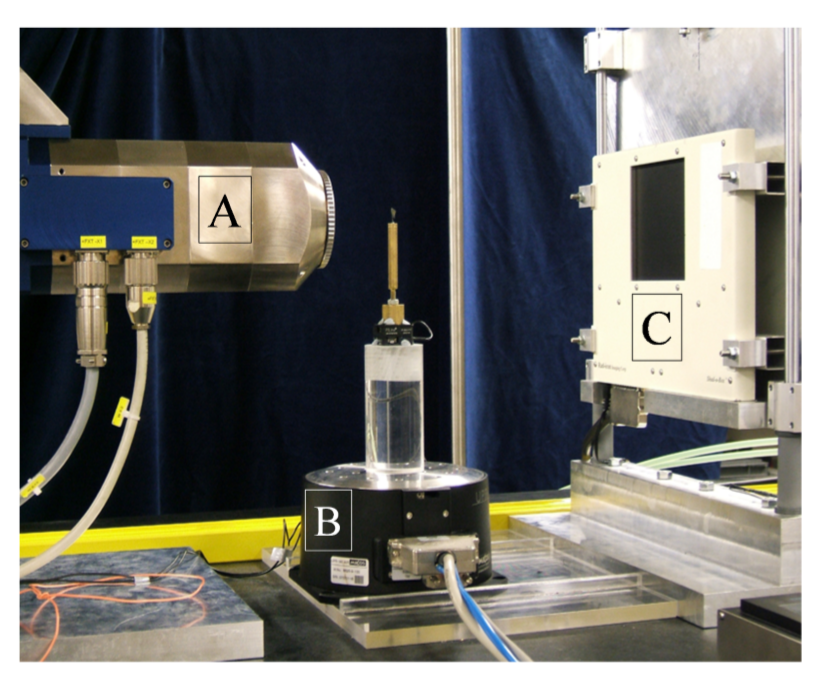
\includegraphics[width=1\textwidth]{\dir/figs/edinburghxray.png}
  \caption{ECOSSE X-ray μCT scanner components: (A) X-ray source (Feinfocus dual head transmission/directional nano/microfocus tube), (B) Air-bearing rotary table (Micos UPR-160F SMC pegasus with taurus motion controller), and (C) 4 MP Gadox X-ray camera (Rad-icon Shad-O-Box)}
  \label{edinburghxray}
\end{figure}

Projection data was acquired via a local C++ code and operated via a Testpoint (V.6) Shell program to coordinate the table rotation with image sensor.

Subsequent image reconstruction was performed via Octopus\texttrademark. The high grey scale contrast between brine and crude or mineral oil enabled direct thresholding segmentation of discrete fluids and rocks. Data analysis and visualisation were using Avizo9\texttrademark and ImageJ software.

%##################################################################################